\pagebreak
\section{Experiment 4}
In this experiment the relationship between class separability and error probability is explored by creating 10 pairs of 2-class datasets, each separated monotonically such that the Mahalanobis distances for each pair of classes were recorded as: $d_{M}^{2} = 1.45, 1.7, 3.4, 3.7, 4.583, 6.25, 12.5, 12.75, 16.67, 24.05$. These classes were generated randomly and then sorted to ensure that the sequence of class pairs would be ranked in a monotonic fashion (and manually checked so as to not be equal). All the class parameters were randomized in this experiment, and the covariance matrix was some randomized diagonal matrix. The number of test samples was nominally chosen as 100 samples per class to remain consistent with much of the other experimentation in this report.

\subsection{Results \& Discussion}
What can be observed in the results is that in general as the Mahalanobis distance between the two classes increases, its linear separability is increased, naturally leading to reduced errors. This is reflected in Figure \ref{fig:exp4} in which there is a distinct downward trend in the error percentage as a function of the Mahalanobis distance. There do exist some occasional upwards spikes in error which can likely be attributed to individual test case variations, as in this experiment 10 iterations per sequence was not performed (unlike in previous experiments). This makes it more prone to noise and extrapolating from previous experiments (1 and 2), adding this iterative step to aggregate a mean error would reduce the sensitivity to such spikes.

\begin{figure}[H]
	\centering
	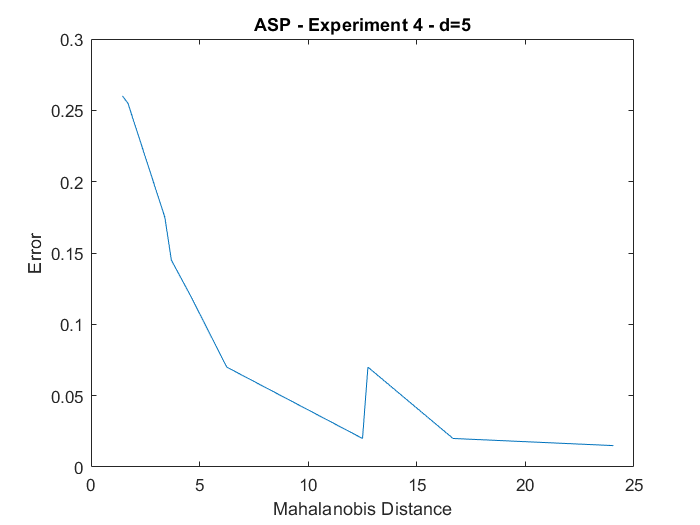
\includegraphics[width=.9\linewidth]{./code/Exp4-results/MahalError_d5_s10.png}
	\caption{Experiment 4 Results}
	\label{fig:exp4}
\end{figure}
